\documentclass{llncs}
%\documentclass[a4paper]{article}

%\usepackage{fullpage}
\usepackage{setspace}
\usepackage{url}
\usepackage{algorithmic}
\usepackage{algorithm}
\usepackage{amsmath}
\usepackage{latexsym}
\usepackage{multirow}

\usepackage{graphicx}
\usepackage{subfig}

%\onehalfspacing

%\newtheorem{definition}{Definition}
%\newtheorem{theorem}{Theorem}
%\newtheorem{example}{Example}
\newtheorem{query}{Query}

\newcommand{\nop}[1]{}

\setlength{\tabcolsep}{2pt}

\newcommand{\myremark}[2]{{\textbf{\marginpar{$\parallel$}(* \textit{#1:} #2 *)}}}
%\newcommand*\justify{%
%  \fontdimen2\font=0.4em% interword space
%  \fontdimen3\font=0.2em% interword stretch
%  \fontdimen4\font=0.1em% interword shrink
%  \fontdimen7\font=0.1em% extra space
%}


\title{Mapping Microblog Posts to Encyclopedia Articles}
\author{Uta L\"{o}sch \and David M\"{u}ller \and Andreas Harth}
\institute{Institute AIFB, Karlsruhe Institute of Technology (KIT), Germany\\ 
	\email{uta.loesch@kit.edu},\\
	\email{david.mueller@student.kit.edu},\\
	\email{harth@kit.edu}
}
\begin{document}

\maketitle

\begin{abstract}
Microblog posts may contain so-called hashtags that mark keywords or topics.
Hashtags are used in an ad-hoc fashion; the meaning of hashtags is implicitly defined via their use, which makes understanding and querying hashtags difficult.
In this paper we devise a method for annotating microblog posts which contain hashtags with related encyclopedia entities.
Thus, users have the means to quickly grasp the meaning of a hashtag, and gain starting points for further exploration of the hashtags' context.
We implement two variants of our method based on an existing system for linking content to Wikipedia and analyse the stability of annotated  Twitter search results for popular hashtags.
\end{abstract}

\nop{
Keywords: Twitter, Wikipedia, DBpedia, RDF

http://tagdef.com/ has a list of popular tags
}

\section{Introduction}

Microblogging services allow users to publish short messages online.
Twitter\footnote{\url{http://twitter.com/}} is the largest dedicated microblogging site; as of March 2011, its users create an average of 140 millions post a day\footnote{\url{http://blog.twitter.com/2011/03/numbers.html}}.
Given a 140-character limit for posts, Twitter users invented shortcuts for certain expressions.
So-called hashtags (starting with a \# sign followed by a keyword) are frequently used to associate posts with a specific topic, place, person or event.
For example, posts covering current events in Lybia are frequently tagged with $\#Libya$.
%the Extended Semantic Web Conference 2011 will frequently be tagged with $\#eswc2011$.

Hashtags can help to organise microblog messages and thus are useful for supporting search.
Microblogging platforms offer functionality to search for messages containing a specific hashtag.
%This search returns the most recent messages containing the tag.
However, as hashtags are implicitly defined via their use, the meaning of a hashtag is often unclear.
Services such as tagdef\footnote{\url{http://www.tagdef.com/}} provide means to provide a definition of a hashtag, but these services rely on user input and thus only cover a subset of all hashtags.
In addition, since hashtags are not related to other structured information sources, querying is limited to direct keyword search.

We propose a method to associate hashtags to encyclopedia entities.
In our experiments we use Wikipedia as entity source which covers a wide range of topics.
Furthermore, automatic tools for annotating text with Wikipedia entities are readily available, for example Milne and Witten's Wikifier \cite{key:wikifier}.
Wikipedia entities are widely linked to external data sources via DBpedia \cite{key:dbpedia}, thus combined querying of DBpedia and Twitter becomes possible.

Matching entities in microposts is a difficult problem \cite{key:clef} as microblog post are very short and contain little information.
Our approach uses search results for a given hashtag as input to the entity matching component and returns messages using the hashtag including a set of related Wikipedia entities.
% which have been detected in the search result.
The matched entities not only help to understand the search terms, but also serve as a starting point for refining the search or searching for further information related to the search result.
%These entities will help the user to gain an understanding in which context the hashtag is used and what it may mean.

%with a set of entities which reflect the content of the result feeds.
%, it is necessary to parse the whole set in order to get an overview of the context(s) in which the search term is used.
%grasp the context of the results and to get further information on the topic that was searched for.
%To facilitate this putting into context of the search results, 
%Furthermore, this annotation will help to understand hashtags. 
%If users encounter this hashtag and do not understand it, they can search for it on the microblogging platform.
%However, understanding a search result is difficult and time-consuming.

\nop{
Finding entities matching a query, especially a query for a given hashtag is difficult as little context is available due to the short length of each single message.
}

In this paper, we present a method to automatically annotate hashtag search results with encyclopedia entities.
If a hashtag can be associated with an entity with high confidence, the entity can be seen as descriptive for the hashtag.
We envision a system which automatically finds entities equivalent to a hashtag.
%While it would be more interesting to annotate each single microblog message with relevant entities, microblog messages are too short to contain much relevant information which could be used as input for an annotation tool such as the Wikifier \cite{key:wikifier}.
%Thus, we chose to generate annotations for the whole search result. 
%Our implementation is based on Twitter, the most widely used and biggest microblogging platform, and on Wikipedia.
Annotations should be stable over time, unless the topics discussed in the microblog messages containing the search term change.
In an evaluation of our approach we analyse the stability of the results of the entity matching for hashtag search results.

Our contributions thus are:
\begin{itemize}
	\item We present an approach for finding entities which are related to search results on microblogging platforms.
%	\item We specify a formatting of microblogging messages as RDF.
	\item We evaluate the stability of the found entities.
\end{itemize}

The remainder of this paper is organised as follows: Section~\ref{sect:method} overviews the approach,
Section~\ref{sect:impl} presents the implementation,
Section~\ref{sect:eval} covers the results of the evaluation,
Section~\ref{sect:relWork} discusses related work and  Section~\ref{sect:conclusion} concludes.

\section{Method Overview}
\label{sect:method}

The goal of our method is, given a search query $q$ as input, to provide the user with an RDF\footnote{\url{http://www.w3.org/RDF/}} document describing the search result $R$, i.e. the most recent messages that match the query, the authors of these messages and the most relevant entities $E$ for this result. 
In the following we will illustrate our approach based on a search for the hashtag $\#Libya$, a hashtag
which is frequently used to describe posts related to the country of Libya.

The architecture of our proposed system is shown in Figure~\ref{fig:arch}. Upon
receipt of a query $q$ four steps are performed. 

\begin{figure}[htb]
  \centering
  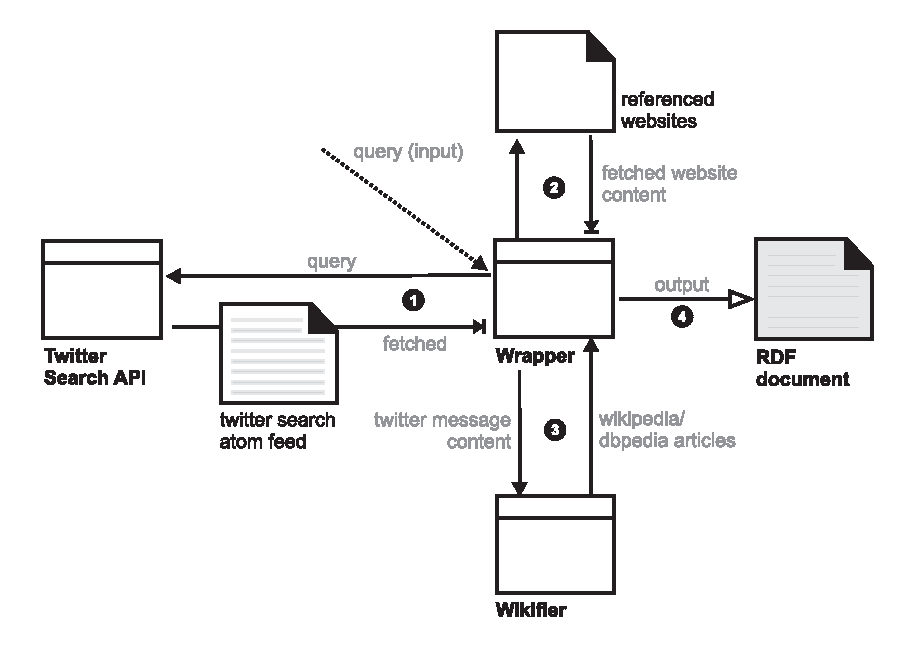
\includegraphics[width=.7\linewidth]{architecture}
  \caption{System Architecture}
  \label{fig:arch}
\end{figure}

\begin{enumerate}
	\item In a first step, the most recent search results $R$ for the query are
	obtained.\newline In our example, calling the Wrapper with query $\#Libya$ will
	return a document containing all most recent Twitter posts whose content
	matched the search string $\#Libya$ and their meta information. 
	\newline
	An example\footnote{\url{http://twitter.com/SenJohnMcCain/statuses/46619460060196865}}
for a single retrieved post is the following:
{\small
\begin{verbatim}
"Arab League calls for no-fly zone in #Libya http://t.co/ZsLNIWa"
\end{verbatim}}
This message posted by Twitter user \texttt{SenJohnMcCain}; geo coordinates\footnote{The original Twitter message posted by SenJohnMcCain was not geo-tagged} and the date the message has been posted are furthermore known.
  
  \item In a second (optional) step hyperlinks posted in messages of the fetched
  feed are followed, content of the referenced website is fetched and processed by the Wrapper. The idea is to acquire additional content which is used as additional signal when searching for entities. We have thought of other methods for enriching the result, like searching for other messages posted by users which have posted messages in the result set. However, these alternative methods are more likely to introduce noise in the signal which is used for obtaining relevant entities.
  
In our example, the message contains a link to
\url{http://t.co/ZsLNIWa}, which redirects to an article on the situation in
Libya published on \url{http://reuters.com/}. Dereferencing this URL and grabbing
the text found at the link should return the following text:
{\small\begin{verbatim}"Arab League calls for Libya no-fly zone-state TV - CAIRO, March 12
(Reuters) - The Arab League on Saturday called on the U.N. Security 
Council to impose a no-fly zone on Libya, Egyptian state television
reported, a decision that would give a regional seal of approval
that NATO has said is needed for any military action."\end{verbatim}}
	\item In a third step entities matching the search result are retrieved. The
	content of the Twitter messages that matched the search query and, if available, the content of referenced websites is merged to a single input string and used as input for the annotation. The result of this step is a list of matching articles of the English Wikipedia.

In our example, the contents of all posts related to the search term '\#Libya'
are merged with the retrieved external website content. Thus, the post obtained from
step 1 would be matched with the website content obtained in step 2 into a
single input stream:
\begin{verbatim}"Arab League calls for no-fly zone in #Libya
Arab League calls for Libya no-fly zone-state TV - CAIRO, 
March 12 (Reuters) - The Arab League on Saturday called on the 
U.N. Security Council to impose a no-fly zone on Libya, 
Egyptian state television reported, a decision that would give
a regional seal of approval that NATO has said is needed for 
any military action."
\end{verbatim}
This string is appended to the Twitter content and the external content of all other posts in the result.

In the example, we would expect to find entities which are related to Libya,
like Libya, Gaddafi or the Arab\_League.

	\item	Finally, an RDF document is generated representing the search results and
	the annotations. Continuing our example, the output RDF document should contain the following
	triples to reference the DBPedia mappings:
	{\small\begin{verbatim}	<http://km.aifb.kit.edu/services/twittersearchwrap/searchwrap
	?q=\%23lybia>
     rdfs:seeAlso <http://dbpedia.org/resource/Lybia> ,
        <http://dbpedia.org/resource/Gaddafi> ,
        <http://dbpedia.org/resource/Arab\_League> .\end{verbatim}}
	The Twitter posts matching the search term \#Libya are likewise all described
	in the output document. The description for the post from our example 
	%abbreviated \texttt{m} 
	results in the following triples:
	{\small\begin{verbatim}<http://km.aifb.kit.edu/services/twitterwrap/statuses/
	show/46619460060196865\#id> 
	   foaf:page <http://twitter.com/SenJohnMcCain/statuses/
	      46619460060196865>;
	   dc:date "2011-03-12T17:12:00Z" ;\newline geo:lat "49.010239" ;
	   geo:long "8.411879" ;
	   foaf:maker <http://km.aifb.kit.edu/services/twitterwrap/users/
	      show?screen\_name=SenJohnMcCain\#id> ;
	   dc:description "Arab League calls for no-fly zone in \#Libya 
	      http://\newline t.co/ZsLNIWa" . \end{verbatim}}     
\end{enumerate}

\section{Implementation}
\label{sect:impl}

We provide an implementation of our approach in the Twitter Search Wrapper\footnote{Online at \url{http://km.aifb.kit.edu/services/twittersearchwrap/}}.

The implementation is based on a set of existing components: 
\begin{itemize}
\item Twitter search results are obtained by using the Twitter search API\footnote{\url{http://dev.twitter.com/doc/get/search}}, a RESTful API which delivers search results in JSON. The result is a feed containing the 100 most recently published Twitter messages, which are publicly visible and match the query, and their authors. The messages themselves are described by their content, publishing date, authors
and optionally a geographic location.

\item The optional step of dereferencing URLs which are posted in messages contained
in the result set can be triggered using the option \texttt{extern=true}. To keep the input size for the next steps manageable, only the first 50 words of the referenced sites are used. The content
retrieved from external websites is beautified for our purpose removing
HTML-tags and scripting elements using the CyberNeko Java HTML Parser
Library\footnote{\url{http://sourceforge.net/projects/nekohtml/}}.

\item The Wikifier \cite{key:wikifier} is used for obtaining content annotations. This tool takes a text as input and returns a set of Wikipedia entities which are relevant for the analysed text. It represents a state-of-the-art annotation tool and was chosen as it allows for finding entities not from some tool-specific knowledge base but from DBpedia, which is one of the most widely used data sources on the Linked Data Web.

\item The system generates and outputs an RDF document in RDF/XML Syntax containing a
description of the retrieved messages matching the search query for the given query and references to the DBpedia articles that have been returned by the Wikifier. 
%It describes the result by means of the popular vocabularies FOAF \cite{key:foaf}, Dublin Core\footnote{\url{http://dublincore.org/documents/dcmi-terms/}}, the Basic Geo Vocabulary \cite{key:geo}. A single Twitter message is described by its individual page using the \texttt{foaf:page} predicate. The date and time the message has been posted is specified using the \texttt{dc:date} predicate. The message's content is annotated using \texttt{dc:description}, while the geographic location of the message is indicated by \texttt{geo:lat} and \texttt{geo:long} predicates. The creator of the Twitter message is referenced by \texttt{foaf:maker} predicate which points to a service that uses RDF to describe information related to a Twitter user which has previously been implemented here at the institute as the message creators URI.

The annotations are added to the search result using \texttt{rdf:seeAlso} links to DBpedia entities \cite{key:dbpedia} which are obtained by a direct transformation of the Wikipedia entities' URLs. DBpedia has been chosen as these entities allow for a more coherent presentation of the content in the context of RDF.

\end{itemize}

%The example Twitter message given in the previous section is represented in
%the output of the Twitter Search Wrapper as follows:\newline
%\linebreak
%\texttt{<rdf:Description
%rdf:about="http://km.aifb.kit.edu/services/\newline
%Twitterwrap/statuses/show/1234567890\#id">\newline
%	<foaf:page
%	rdf:resource="http://Twitter.com/sample\_user\_12345/\newline
%	statuses/1234567890"/>\newline
%	<dc:date>2011-02-23T12:00:00Z</dc:date>\newline
%	<geo:lat>49.010239</geo:lat>\newline <geo:long>8.411879</geo:long>\newline
%	<foaf:maker
%	rdf:resource="http://km.aifb.kit.edu/services/\newline
%	twitterwrap/users/show?screen\_name=sample\_user\_12345\#id"/>\newline
%	<dc:description>\newline Just returned from a wonderful holiday in \#ka.
%	\url{http://www.karlsruhe.de/stadt/tourismus.en} @KarlsruheTweets\newline
%	</dc:description>\newline
%	</rdf:Description>\newline}
%	\linebreak
%Furthermore the mappings to DBpedia articles returned by the Wikifier
%are represented in the output document. In the Twitter Search Wrapper the
%representation is done the following way, again using the introductory
%example from the previous section:\newline
%\linebreak
%	\texttt{<rdf:Description rdf:about=""/>}\newline
%	\texttt{<rdfs:seeAlso
%	rdf:resource="http://dbpedia.org/resource/Karlsruhe"/>}\newline
%	\texttt{<rdfs:seeAlso
%	rdf:resource="http://dbpedia.org/resource/Germany"/>}\newline
%	\texttt{<rdfs:seeAlso rdf:resource="http://dbpedia.org/resource/\newline
%	Karlsruhe\_Institute\_of\_Technology"/>}\newline
%	\texttt{</rdf:Description>}\newline

\section{Experiments and Evaluation}
\label{sect:eval}

We have evaluated our approach to assess whether the entities which are found as related to a specific hashtag are stable over time.

\subsection{Setup}

We have conducted experiments on a set of queries which were identified to be hashtags which are frequently used on Twitter.
To obtain these, we have sampled the Twitter message feed using Twitter's
Streaming API for one minute twice an hour from 2011-03-03 to 2011-03-06. The
top-50 hashtags derived from the aggregate sample are listed in Table
\ref{tbl:hashtags}, count is the number of times we encountered them during the
collection period.



\begin{table}[ht*]
\centering
\small
\begin{tabular}{ l|l|l|l|l|l|l|l|l }
Hashtag & Count & $N_{ext}$ & $E(aut)$ & $Var(aut)$ & $E(ts)$ & $Var(ts)$ & $E(ts_{ext})$ & $Var(ts_{ext})$\\
\hline
\#ff &     460 & 48 & 2.2936 & 0.7014 & 0.1268 & 0.0681 & 0.2037 & 0.0281 \\
\#np &     172 & 48 & 0.4737 & 0.0287 & 0.0655 & 0.0196 & 0.0717 & 0.0195\\
\#nowplaying & 144 & 17 & \textbf{0.4514} & \textbf{0.0251} & 0.0565 & 0.0198 & 0.0458 & 0.0212 \\
\#winning &     134 & 48 & 0.8236 & 0.2365 & 0.1101 & 0.0666 & 0.1816 & 0.0272 \\
\#fb & 105 & 1 & 1.1705 & 1.1826 & 0.1083 & 0.0933 & -- & -- \\
\#rt & 83 & 48 & 1.7980 & 3.7309 & 0.0979 & 0.0763 & 0.1487 & 0.0267 \\
\#mentionke & 61 & 48 & 7.5459 & 195.6829 & 0.1406 & 0.0921 & 0.2215 & 0.0408 \\
\#blackpeoplemovies & 57 & 3 & 90.6195 & 2007.5551 & 0.3327 & 0.0606 & 0.0349 & 0.0244\\
\#tigerblood & 56 & 48 & 3.4029 & 4.8740 & 0.1497 & 0.0692 & 0.2330 & 0.0278 \\
\#thataintwinning & 53 & 48 & 16.8075 & 236.8694 & 0.0768 & 0.0435 & 0.1668 & 0.0387 \\
\#fail & 53 & 48 & 2.3356 & 2.0669 & 0.1927 & 0.1517 & 0.1073 & 0.0460 \\
\#teamfollowback & 52 & 48 & 0.9269 & 0.4871 & 0.1912 & 0.0932 & 0.1813 & 0.0245 \\
\#iftwitterwashighschool & 51 & 48 & 114.8342 & 1771.4564 & 0.5113 & 0.0405 & 0.5144 & 0.0352 \\
\#bieberfact & 51 & 48 & 11.0126 & 63.0455 & 0.0587 & 0.0290 & 0.0765 & 0.0270 \\
\#news & 46 & 0 & 1.8696 & 0.1943 & 0.1024 & 0.0210 & -- & --  \\
\#jobs & 45 & 0 & 1.3866 & 0.4198 & 0.1006 & 0.0192 & -- & -- \\
\#libya & 44 & 1 & 16.0309 & 117.2024 & 0.2701 & 0.0427 & -- & -- \\
\#followmejp & 44 & 0	& 1.5398 & 0.1255 & 0.0688 & 0.0410 & -- & --\\
\#partiu & 41 & 48 & 7.5809 & 84.0531 & 0.6042 & 0.2391 & 0.5313 & 0.2438 \\
\#sougofollow & 39 & 0 & 2.1010 & 0.1820 & 0.0720 & 0.0427 & -- & -- \\
\#damnitstrue & 39 & 48 & 5.7507 & 16.5725 & 0.1805 & 0.1387 & 0.2177 & 0.1579 \\
\#tilltheworldends & 37 & 48 & 85.4526 & 1366.8588 & 0.5682 & 0.0709 & 0.5116 & 0.0324 \\
\#soalcinta & 35 & 48 & 8.4143 & 103.7817 & 0.3451 & 0.1987 & 0.3120 & 0.2014 \\
\#nicovideo & 35 & 0 & 51.0720 & 5521.3529 & 0.3604 & 0.1893 & -- & -- \\
\#quran & 33 & 48 & 45.8290 & 90.4157 & 0.4271 & 0.0501 & 0.4188 & 0.0387 \\
%\end{tabular}
%\begin{tabular}{ l|l|l|l|l|l|l|l|l }
%Hashtag & Count  \\
%\hline
\#nw & 32 & 48 & 2.6054 & 2.1094 & 0.0672 & 0.0231 & 0.0901 & 0.0418 \\
\#quote & 31 & 48 & 4.3007 & 0.5706 & 0.1074 & 0.0197 & 0.1012 & 0.0212 \\
\#shoutout & 30 & 48 & 2.6030 & 3.3256 & 0.2347 & 0.0987 & 0.2526 & 0.0488 \\
\#jfb & 30 & 48 & 23.9911 & 1453.3113 & 0.2483 & 0.1654 & 0.2158 & 0.1379 \\
\#carnaval & 27 & 48 & 34.2574 & 1100.9818 & 0.3229 & 0.2134 & 0.2578 & 0.1646 \\
\#tfb & 26 & 48 & 2.5994 & 0.8777 & 0.2292 & 0.1766 & 0.1760 & 0.0319 \\
\#followme & 26 & 0 & 3.2194 & 0.4650 & 0.1209 & 0.0952 &	-- &	-- \\
\#followfriday & 25 & 48 & 13.6749 & 20.0701 & 0.1910 & 0.1152 & 0.2060 & 0.0676 \\
\#follow & 24 & 48 & 3.0945 & 1.9622 & 0.2916 & 0.1927 & 0.2046 & 0.0305 \\
\#egypt & 23 & 16 & 3.1850 & 3.2745 & 0.1357 & 0.0239 & 0.0704 & 0.0263 \\
\#retweet & 22 & 48 & 4.6991 & 13.4434 & 0.1570 & 0.1232 & 0.1353 & 0.0306 \\
\#fact & 22 & 48 & 5.5613 & 12.0766 & 0.0915 & 0.0762 & 0.0783 & 0.0612 \\
\#win & 20 & 0 & 4.2949 & 5.1856 & \textbf{0.0347} & 0.0221 & -- & -- \\
\#tweetmyjobs & 20 & 0 & 35.5697 & 1590.6997 & 0.3244 & 0.0621 & -- & -- \\
\#music & 20 & 1 & 4.4665 & 4.6392 & 0.0833 & 0.0196 & -- & -- \\
\#in & 20 & 3	& 8.2367 & 6.8944 & 0.0649 & 0.0236 & \textbf{0.0251} & 0.0206 \\
\#imagine & 20 & 48	& 8.3378 & 30.4317 & 0.2465 & 0.1759 & 0.1813 & 0.1375 \\
\#nowwatching & 19 & 48 & 7.9110 & 8.6833 & 0.0672 & 0.0214 & 0.1293 & 0.0211 \\
\#cumannanyaindonesia & 19 & 48 & 77.9680 & 2739.7782 & 0.3901 & 0.1885 & 0.4323 & 0.2033 \\
\#twexit & 18 & 48 & 12.5672 & 255.8178 & 0.3125 & 0.2148 & 0.2417 & 0.1783 \\
\#lcv & 18 & 48 & 28.6309 & 477.9193 & 0.4236 & 0.2395 & 0.2813 & 0.1969 \\
\#fui & 18 & 48 & 11.5515 & 165.3850 & 0.4896 & \textbf{0.2447} & 0.4635 & \textbf{0.2448} \\
\#bot &      18 & 1 & 13.3533 &	8.2469 & 0.2708 & 0.1975 & -- & --  \\
\#nemuritsuzuketeshinu & 17 & 48 & \textbf{314.1120} & \textbf{25053.5657} & \textbf{1.0000} & \textbf{0.0000} & \textbf{1.0000} & \textbf{0.0000} \\
\#fato & 17 & 48 & 17.6223 & 569.5627 & 0.1875 & 0.1523 & 0.2353 & 0.1304 \\
\end{tabular}
\caption{Popular hashtags sampled during a three-day period.}\label{tbl:hashtags}
\end{table}


The goal of our evaluation was to examine the stability of the entity annotations over time. To achieve this, we have repeatedly executed the same set of queries and analysed the returned data. 

In principle, two methods for data acquisition were identified: \begin{definition}[Data Acquisition Methods]
\begin{itemize}
\item {\bf Temporal Sliding Window}\newline The query is executed and the $n$
most recent results are retrieved every $t$ minutes. The Temporal Sliding Window
method may lead to duplicate messages in the retrieved documents.
\item {\bf $k$-item Sliding Window}\newline  The $k$-item Sliding Window method
retrieves all messages that match the query exactly one time. Each time $k$ new messages are
available matching the given query a document containing those $k$ messages
is retrieved. This method needs constant monitoring of recently posted messages matching the search term.
\end{itemize}
\end{definition}

The disadvantage of the first method is that it is neither possible to guarantee that all messages matching the search are collected, nor is it possible to avoid overlaps between the search results. However, while the second method seems to overcome these problems, it does not: Using the $k$-item sliding window method, it is not clear when the next search result should be fetched: even when frequently querying for new messages, if updates are frequent it is likely to lack messages in the result set.

For our data set queries were executed twice per hour using the Temporal
Sliding Window method in a 24 hour time frame. Data was
collected on 2011-03-07\footnote{Collected data is available under
\url{http://people.aifb.kit.edu/aha/2011/twittersearch/twittersearch-2011-03-10.zip}}.

\subsection{Measures}

For analysing the collected data, several measures were defined:

\begin{definition}[Evaluation Measures]
Given disjoint result sets $R_1,\ldots,R_n$ for a query $q$ obtained at times $t_1,\ldots,t_n$ and annotated with sets of entities $E_1,\ldots,E_n$, where each result set $R_i$ consists of Twitter messages $r_i1,\ldots,r_iK$ with time stamps $t_i1,\ldots,t_iK$ we define:
\begin{itemize}
	\item The average update time within a result set $aut(R_i)$ for a query is the average time that lies between messages that match the query which produced the search result: $$aut(R_i)=\frac{\sum_{j=1}^{K}t_{i,j+1}-t_{i,j}}{K-1}$$
	A high $aut(R)$ means that new messages that match the query are not generated very often. If new messages matching the query are frequently published, then the $aut(R)$ is low.
	
	The mean $E(aut(q))$ and the variance $Var(aut(q))$ of the $aut(R_i)$ can be used to describe update properties for the result sets that are generated for a given query. E.g. if for a given query $E(aut(q))$ is high and $Var(aut(q))$ is low, then the rate at which messages are published is stable at a quite low level.
%	\item The global stability $gs$ of the results shows how stable the whole set of entity terms for a query is. It is defined as: $$gs(q)=\frac{|\bigcap_{i=1}^{n}E_i|}{|\bigcup_{i=1}^{n}E_i|}$$
%	A value of $gs(q)$ of $1$ means that the set of entities is the same at each point in time $t_i$. On the other hand, a value of $0$ means that at least two of the sets of entities, with which the results were annotated, are disjoint.
	\item The stability for a single term is defined as the fraction of result sets for a query $q$ in which it occurs: 
$$sts(q,t)=\frac{|\{i|t\in E_i\}|}{n}$$
	If the value of $sts$ is $1$ the term occurs in all of the result sets for the query, if it is close to $0$ it occurs in few result sets.
	\item The time stability $ts$ for a query $q$ at time $t_i$ is the fraction of
	entities which are unchanged between the result set at $t_{i-1}$ and $t_i$: 
	$$ts(q,t_i)=\begin{cases} 1 & i=1 \\
														1 & E_{i-1}\cup E_i = \emptyset\\														
														\frac{|E_{i-1}\cap E_i|}{|E_{i-1}\cup E_i|} & i>1\end{cases}$$
	A value of $1$ means that the two sets of entities are identical, a value of $0$ means they are disjoint.
	
	The variance $Var(ts(q))$ of time stabilities $ts(q,t_i)$ over all $t_i$ helps to determine whether the rate at which the found entities change is rather stable or whether it is changing a lot over time.
\end{itemize}
\end{definition}

\subsection{Results}

An overview of the results we obtained for the frequently used hashtags is given in Table~\ref{tbl:hashtags}. The most frequent entities for some of the tags are listed in Table~\ref{tbl:entities}. In total, we have analysed 48 result sets for each of the query tags. However, in some cases, the analysis which includes the content of external web pages led to a timeout of the Wikifier. $N_{ext}$ gives the number of result sets which we could analyse when the external content is included. $E(aut)$ and $Var(aut)$ give the results for analysing the average update times of the result sets. In our analysis estimated $aut$s range from $0.45$ seconds to $314.11$ seconds, i.e. approximately $5$ minutes. In order to avoid any duplicates in the result sets, an average update time of less than $18$ seconds is needed. Note that update times below this value do not guarantee disjointness of the result sets, as the value is only an average, and high update frequencies in one result set may outweigh low update frequencies in other result sets. Additionally, we have analysed the variance of the $aut$s. A low variance means that the update intervals remain relatively stable over time, while a high variance indicates that messages using the hashtag were posted rather irregularly. In general, higher average update times are associated with a higher variance in the update times. In some cases however, the variance of the average update time is surprisingly low when the mean average update time is rather high: this is e.g. the case for the tags $\#bieberfact$, $\#quran$, $\#followfriday$. For these tags updates were published at a relatively regularly.

\begin{table}[ht]
\centering
\small
\begin{tabular}{l|l|l|l|l}
Hashtag & Definition on tagdef.com & Extern & $E$ & $sts$ \\%& $E_2$ & $sts(E_2)$ & $E_3$ & $sts(E_3)$ \\
\hline
\#tilltheworldends & - & false & Britney Spears & .9583 \\
& & &  iTunes & .6875 \\
& & &  itunes & .625 \\ 
\hline
\#tilltheworldends & - & false & Britney Spears & 1 \\
& & &  itunes & .75 \\
& & &  Amazon.com & .5625 \\ 
\hline
\#nowplaying & What people on Twitter & false & iTunes & .5208 \\
             & are currently listening & & Michael Jackson & .333 \\
             & to. & & Lady Gaga & .333 \\
\hline
\#nowplaying & same & true & YouTube & .8235 \\
             &  &  & Hip Hop Music & .6471 \\
             &  &  & The Notorious B.I.G. & .5883 \\
\hline
\#np         & Now playing = \#NP & false & Chris Brown\_(entertainer) & .5 \\
& & & Usher & .3125 \\
& & & Lil Wayne & .2917 \\
\hline
\#np & same & true & Chris Brown\_(entertainer) & .5 \\
& & & YouTube & .375 \\
& & & Ne-Yo & .315 \\
\hline
\#thataintwinning & -& false & Mozilla Firefox & .2291 \\
& & & Twitter & .2291 \\
& & & twitter & .1667 \\
\hline
\#thataintwinning & - & true & twitter & .5208 \\
& & & Twitter & .5 \\
& & & Two and a half men & .125 \\
\hline
\#blackpeoplemovies & - & false & Devil & .4791 \\
& & & Tyler Perry & .2708 \\
& & & Harry Potter & .2292 \\
\hline
\#blackpeoplemovies & - & true & Amazon.com & 1 \\
& & & YouTube & 1 \\
& & & amazon.com & 1
\end{tabular}
\label{tbl:entities}
\caption{Most frequent entities and their single term stabilities}
\end{table}

We also report the average time stability over all time points as well as the variance for each hashtag. A high time stability indicates that more or less the same entities were used for annotation at all times. The highest stabilities were achieved for the tags $\#nemuritsuzuketeshinu$ and $\#partiu$, because no (resp. very few) entities could be associated with the results of this search. This can be explained as the tags are only used in Japanese resp. Spanish Twitter messages. However, the Wikifier analyses the content of the results as being English text. A solution could be to search only for English messages, however, this is not possible as Twitter messages have no language tags and location attributes are no sufficient indicator for the language in which a user will write messages.

The third highest stability was achieved by the tag $\#tilltheworldends$ which refers to Britney Spears' newest single. The different spellings of iTunes which are used for annotation occur as the Wikifier does not return normalised entities.

Very low time stability was obtained for the tag $\#nowplaying$ which is used to tell which song one is currently listening to (a similarly low stability is obtained for the tag $\#np$ which is often used synonymously with $\#nowplaying$). As these messages contain all kinds of artist names and songs names, it is thus expected that the entities which are found vary between the result sets.

The effect of considering external content in the annotation is beneficial in some cases, in others the effect was destabilising. The highest decrease in stability was observed for the tag $\#thataintwinning$, the highest increase occurred for the tag $\#blackpeoplemovies$. Our hypothesis is that de-stabilisation occurs especially in cases where the posted links cover a variety of topics, while for more specific hashtags referenced web sites are more likely to cover a specific topics and will thus be stabilising.

\section{Related Work}
\label{sect:relWork}

Bringing Semantic Web technologies and Semantic Web technologies together, has been proposed several times.

The SemanticTweet\footnote{\url{http://semantictweet.com/}} service is a tool which allows for the generation of a FOAF file describing one's network of followers and friends on Twitter. Thus, an automatic way of mapping the Twitter social network to semantic data is made available. The transformation is syntactic and does not include links to topics.

Passant et al. \cite{key:smob} have proposed a data model for making Twitter data available on the Semantic Web. They propose a data model which allows for the association of URIs with users, microblogs and microposts. To this end, SIOC and FOAF vocabularies are used and extended. Specifically, the new concepts \emph{Microblog} and \emph{MicroBlogPost} are introduced. Additionally, they propose the use of so-called semantic hashtags. The idea is to use URIs as hashtags (e.g. \emph{\#geo:Paris\_France}). It becomes thus possible to link microposts to entities on the Linked Data Web via these semantic hashtags. 
In contrast we do not require users to change their behavior by requiring them to use another type of hashtags. Instead, our method finds DBpedia entities which are related to the query automatically.

Softic et al \cite{key:softic} have developed a framework and system for mining data from social networks. They have instantiated their system to analyse data from Twitter. In their system, they collect data from one or several users. The system by Passant et al. \cite{key:smob} is used for transforming Twitter data to semantic data. The triplified data can then be analysed using SPARQL. They propose that the result data could be enriched using entities from other Linked Open Data vocabularies like DBpedia\footnote{\url{http://dbpedia.org/}} or GeoNames\footnote{\url{http://www.geonames.org/}}, but they do not provide an actual method how this annotation can be achieved.

Relating semantic concepts with Twitter messages has been attempted by various authors:
Stankovic et al. \cite{key:stanko} propose to use the Zemanta\footnote{\url{http://developer.zemanta.com/}} keyword extraction API to detect topics of single Twitter messages. 
% from stakovic et al.
%In order to make tweets more searchable and make them useful for the described
%scenario one would need to have represent them in a structured format and associate
%those tweets with the topics that refer to. As a basic approach we process the text of
%the tweets using Zemanta16 keyword extraction API. This approach gives DBPedia
%concepts related to a tweet, but is useful only on a limited number of tweets directly
%mentioning a particular topic. In the example data set we produced from ESWC2010,
%tweet topics are represented using dc:subject property.
Instead of mining single messages which provide little signal to the extraction algorithm we use an aggregation of messages as input to the extraction component.

Similar to our approach, Wagner \cite{key:clauwa} proposes to use aggregations of social awareness streams for knowledge extraction. As such, our approach is closely related.

Kinsella et al. \cite{key:kinsella} use hyperlinks in posts to derive a richer representation of those posts. We too use external data to augment the set of Twitter messages supplied to the Wikifier system in a variant of our method.

The challenge task in the WePS-3 Online Reputation Management Task\cite{key:clef} requires systems to detect mentions of company names in Twitter messages.
The corpus contains evaluation results solicited via Mechanical Turk. In contrast to the WePS-3 task, we associate generic hashtags to Wikipedia/DBpedia concepts.


\section{Conclusion and Future Work}
\label{sect:conclusion}

We have presented an approach for annotating Twitter hashtags with Wikipedia entities.
We have described an implementation of two variants of the method and evaluated the approach. In an evaluation we have shown that meaningful entities were found for many hashtags and that these entities remain stable over time.

However, our evaluation has shown that a direct mapping of hashtags to a single DBpedia concept is not always possible.
One reason is that hashtags do not necessarily describe an entity, but are rather used to describe contexts.
Another reason is the use of hashtags for different entities.
For example, both the hashtags $\#ka$ and $\#karlsruhe$ are frequently used when talking about topics which are related to the city Karlsruhe.
The tag $\#ka$ is however also used to denote the car type Ford Ka.
Thus, when searching for $\#ka$ on a microblogging platform, messages relating to Karlsruhe will be found as well as messages related to Ford Ka.
An approach which aims at finding relevant entities for a given search will have to be able to disambiguate homonym hashtags.
%deal with these problems.

An issue we have encountered is that different languages have to be dealt with: topics are often commented on in a variety of languages, and the built-in language identifiers are often incorrect.
As the entity matching system is language-dependent we would need to include a language detection component in future versions of the system.

%Note however that a direct mapping of hashtags to entities is not possible in many cases: e.g. there is no entity in DBpedia which describes the Extended Semantic Web Conference 2011, thus the tag $\#eswc2011$ can not be mapped directly.
%Additional problems are due to synonyms and homonyms in the set of hashtags that are frequently used.


%@@@ how to select external data (parse text from HTML, which part of web page to select - boilerplate stuff might spoil the results (reference blog cleansing paper

\bibliographystyle{abbrv}
\bibliography{bib}

\end{document}
